\section{Results}\label{sec:results}

Table~\ref{tab:headline} summarises the audit in the metrics that matter
for reproducibility; the subsections unpack each row. One remark applies
throughout: none of the findings below is a criticism of the benchmark's
authors, whose documentation is far above the norm for the genre and whose
distributed workbook is what made a cell-level audit possible at all. Small
reconciling interventions are a normal and necessary part of SAM
compilation; our findings concern whether the record allows them to be
seen, not whether they should exist.

\begin{table}[t]
\centering\small
\caption{Headline replication metrics: our reconstruction from
publicly obtainable sources, audited against the published benchmark.
Comparisons use the tolerance of Section~\ref{sec:method:terms}
(R0.5~million, the benchmark workbook's rounding grain) unless stated;
``comparable'' cells are those nonzero in both our matrix (6{,}779
nonzero cells) and the benchmark's (6{,}737).}
\label{tab:headline}
\begin{tabularx}{\textwidth}{lXl}
\toprule
Block & Metric & Result \\
\midrule
Production (61 activities) & output, intermediates, prod.\ taxes, VA & exact ($\le$R0.5m), 61/61 each \\
Final demand (5 categories) & per-commodity agreement & exact, all commodities (316/316) \\
Institutional macro (SARB) & 45 computable cells & 43 exact; 45 within 1\%; max 0.139\% \\
Capital split (6 types) & activity--type shares & median 0.18pp; 73.6\% within 1pp \\
Occupation split (10) & activity--occupation shares & median 0.04pp; 88.7\% within 1pp \\
Household groups (14) & wage-income anchor & mean 0.74pp; max 1.9pp \\
Full matrix (209 accounts) & 6{,}732 comparable cells & 62.5\% equal within R0.5m \\
Balanced SAM (v0.2) & max account imbalance & R7m; RAS factors in $[0.907, 1.143]$ \\
\midrule
Non-public inputs & count; priced effect of proxy & 1; mtx $+16.1$\%, stx $-1.5$\% \\
Divergences (record vs.\ data) & catalogued in five classes & 8 (Sec.~\ref{sec:discussion}; App.~\ref{app:evidence}) \\
\bottomrule
\end{tabularx}
\end{table}

\subsection{The production and commodity blocks reproduce exactly}
\label{sec:results:production}

Aggregating the official supply and use tables through the published
concordances reproduces the benchmark's production side to within
R0.5~million on \emph{all} 61 activities: gross output, intermediate
consumption, production taxes, and value added at factor cost each deviate
by 0.0000\,per\,cent. Final demand reproduces exactly per commodity in
every category (households 93/93 commodities, government 3/3,
exports 97/97, fixed capital formation 21/21, and
inventories-plus-residual 102/102---316/316 in all,
confirming that the benchmark's stock-change account absorbs the use
table's residual column). The benchmark matrix itself is exactly balanced
(maximum $|$row$-$column$|$ gap below R0.001~million across the 210
accounts of its distributed matrix; the comparison below is on the 209
accounts of our rebuild). For the macro comparison of
Section~\ref{sec:results:macro} the benchmark is aggregated to the
technical note's Table-2 accounts, the margin account consolidating away
exactly.

Three discrepancies had to be resolved to get there, and each is a finding
about naming rather than about numbers. The account \texttt{atx} carries an
activity-style prefix but is taxes on production (it equals the use table's
$D2/3$ exactly on 61 of 61 activities); the accounts \texttt{cler} and
\texttt{craf} carry the commodity prefix but are the clerical and craft
\emph{occupation} accounts---before reclassification they masquerade as a
systematic R479~billion overstatement of intermediates spread across every
activity; and the value-added comparison closes only at factor cost, since
the benchmark parks production taxes outside its factor payments. The
workbook's own dictionary sheet later confirmed all three
identifications---and added a fourth: the descriptions of the capital
accounts \texttt{mach}, \texttt{nitc}, and \texttt{trnp} are rotated by one
position relative to the technical note's authoritative list.

\subsection{The institutional macro block from SARB series}
\label{sec:results:macro}

Evaluating the technical note's 46 macro cell formulas over the December
2022 SARB Quarterly Bulletin series reproduces 43 of the 45 computable
cells exactly; all 45 are within 1\,per\,cent and the largest deviation is
0.139\,per\,cent. (Of the 46 cells, 43 evaluate directly from KBP-series
formulas and two are defined residually from the others---together the 45
``computable'' cells---while the 46th depends on the unpublished customs
input priced below.) Getting there required three corrections that are
themselves results:

\begin{itemize}
  \item \textbf{A garbled formula, uniquely recovered.} No signed
  combination of the six series quoted for the intra-enterprise cell
  reproduces the benchmark. Searching all $3^6$ coefficient vectors in
  $\{-1,0,1\}$ yields exactly one exact solution---with different signs than
  the prose and one quoted series unused---and the next-best candidate
  misses by R2.5~billion.
  \item \textbf{The unpublished input, priced.} The product-tax cells
  subtract the benchmark's unpublished customs figure (R48{,}934m), not the
  public series the note cites (KBP4590J, R56{,}805m); the note itself
  prints both variants in different places. Under the public proxy, import
  duties deviate by $+16.1$\,per\,cent and product taxes by
  $-1.5$\,per\,cent---the total measured cost, in this SAM, of its one
  non-public input.
  \item \textbf{An unrecorded reconciling adjustment.} Twin gaps of exactly
  $-$R596~million appear in the two government--enterprise cells. A
  data-revision explanation is tested and set aside (the June and December
  2022 bulletins carry identical values for every series involved). Adding
  $+596$ to both directions of a bilateral flow is the unique minimal edit
  that preserves both accounts' balances, so the pattern is consistent with
  a routine reconciling adjustment made during compilation and not recorded
  in the note---exactly the kind of small, legitimate intervention that
  cell-level provenance would turn from a discovery into a declaration.
\end{itemize}

Table~\ref{tab:macro} reports the cells where these three findings act,
under both scenarios; all other computable cells are exact.

\begin{table}[t]
\centering\small
\caption{Institutional macro cells requiring correction or judgment
(R~million; deviations against the benchmark). ``Proxy'' replaces the
unpublished customs figure with the public series KBP4590J.}
\label{tab:macro}
\begin{tabular}{llrrrr}
\toprule
Entry & Cell (receiver $\leftarrow$ payer) & Computed & Benchmark & Dev.\ \% & Proxy dev.\ \% \\
\midrule
vi & stx $\leftarrow$ commodities & 519,805 & 519,805 & +0.00 & -1.51 \\
vii & mtx $\leftarrow$ commodities & 48,934 & 48,934 & +0.00 & +16.09 \\
xv & enterprises $\leftarrow$ enterprises & 857,644 & 857,644 & +0.00 & +0.00 \\
xvii & government $\leftarrow$ enterprises & 428,816 & 429,412 & -0.14 & -0.14 \\
xxviii & enterprises $\leftarrow$ government & 686,931 & 687,527 & -0.09 & -0.09 \\
xxxiv & government $\leftarrow$ stx & 519,805 & 519,805 & +0.00 & -1.51 \\
xxxv & government $\leftarrow$ mtx & 48,934 & 48,934 & +0.00 & +16.09 \\
\midrule
\multicolumn{6}{l}{\emph{Remaining 39 cells: exact (43 of 45 computable within 0.01\%)}} \\
\bottomrule
\end{tabular}

\end{table}

\subsection{Share systems: recovery and honest residuals}
\label{sec:results:shares}

\textbf{Capital.} The technical note specifies neither the AFS edition nor
the stock measure behind its six-way capital split. Grid-testing editions
$\times$ carrying-value columns leaves \emph{2019 revised, closing
values} as the only candidate in the grid consistent with the benchmark
(median share deviation 0.18~percentage
points; 73.6\,per\,cent of activity--type shares within 1pp), against
0.72pp for the preliminary edition that the AFS 2019 publication page
supplies by default. Residual outliers are concentrated and interpretable:
posts and telecommunications deviates by up to 34pp on network equipment,
consistent with a sector-specific reclassification made during compilation
and not reported in the note; and six
activities (agriculture, education, financial intermediation, insurance,
public administration, non-observed) are absent from the AFS altogether, so
their published splits rest on undocumented sources.

Table~\ref{tab:grid} shows the recovery grid.

\begin{table}[t]
\centering\small
\caption{Grid recovery of the capital split's undocumented basis: agreement
with the benchmark's activity--type shares by AFS edition and stock
measure.}
\label{tab:grid}
\begin{tabular}{llrr}
\toprule
AFS edition & Stock measure & Median $|$diff$|$ (pp) & Within 1pp (\%) \\
\midrule
2019 preliminary & opening & 1.05 & 49.1 \\
2019 preliminary & closing & 0.72 & 57.9 \\
2019 revised & opening & 0.72 & 58.2 \\
2019 revised & closing $\leftarrow$ recovered & 0.18 & 73.6 \\
\bottomrule
\end{tabular}

\end{table}

\textbf{Occupations.} Implementing the note's wage-bill procedure on the
LMD microdata reproduces the benchmark's $10\times61$ occupation shares
with median deviation 0.038pp (mean 0.86pp; 88.7\,per\,cent of 610 shares
within 1pp; maximum 24pp in two small-sample industries). A methodological
aside earns its keep here: our own first pass silently dropped the
private-households industry---6{,}202 observations and the home of the
domestic-worker occupation---because a parser assumed three-digit industry
codes. The pipeline's coverage assertion caught it; conventions failed
symmetrically on both sides of the audit.

\textbf{Households.} Two dictionary-free anchors test the benchmark's
group definition, and they disagree---informatively. The wage-income
anchor identifies \emph{household-level} expenditure deciles (top decile
in five 2\,per\,cent bands): under that definition the LCS wage-income
distribution matches the benchmark's labour-to-household block at mean
0.74pp (max 1.9pp), while per-capita grouping fits markedly worse (mean
1.8pp, max 7.9pp). The consumption anchor cannot corroborate it: it fits
poorly under the household-level grouping (up to 5.9pp) and in fact sits
closer to the per-capita alternative (mean 0.71pp against 1.46pp). The
note itself explains why the consumption block is uninformative here: its
consumption shares were carried over from an earlier SAM rather than
recomputed from the LCS---inherited provenance that a fresh, documented
build cannot and should not reproduce, and that decouples the consumption
pattern from whichever grouping the income side uses. The identification
therefore rests on the wage anchor alone.

Table~\ref{tab:occ} details the occupation system by occupation, and
Figure~\ref{fig:ecdf} plots the full distribution of share deviations for
the two microdata-based systems: the mass of both distributions sits far
below one percentage point, with thin, interpretable tails.

\begin{table}[t]
\centering\small
\caption{Occupation shares versus the benchmark, by occupation
(deviations in percentage points across 61 activities).}
\label{tab:occ}
\begin{tabular}{lrrr}
\toprule
Occupation & Median $|$diff$|$ (pp) & Max (pp) & Within 1pp (of 61) \\
\midrule
Managers & 0.340 & 19.02 & 42 \\
Professionals & 0.068 & 24.40 & 50 \\
Technicians & 0.065 & 16.13 & 53 \\
Clerks & 0.080 & 14.94 & 53 \\
Service and sales & 0.028 & 10.01 & 54 \\
Skilled agriculture & 0.000 & 0.84 & 61 \\
Craft & 0.061 & 17.26 & 55 \\
Plant/machine operators & 0.063 & 10.27 & 55 \\
Elementary & 0.087 & 22.81 & 58 \\
Domestic workers & 0.000 & 1.28 & 60 \\
\bottomrule
\end{tabular}

\end{table}

\begin{figure}[t]
\centering
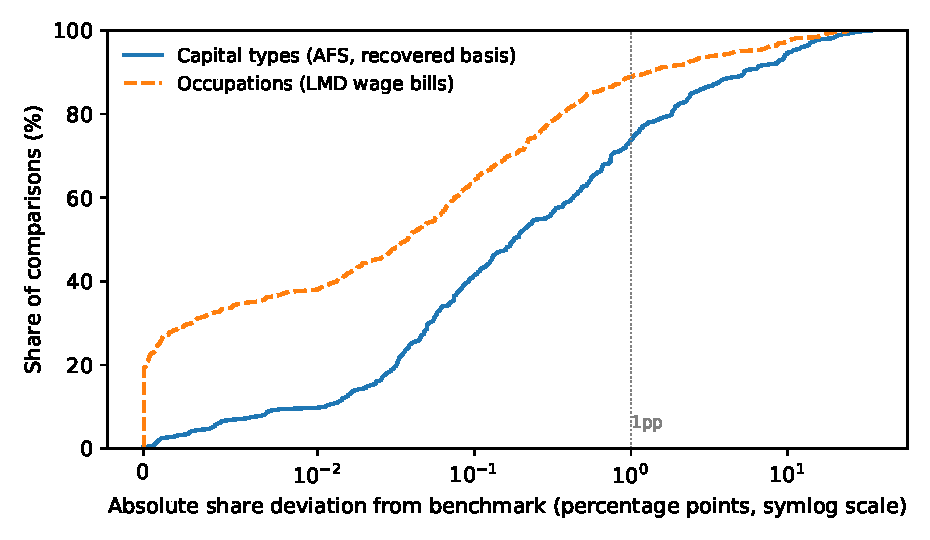
\includegraphics[width=.92\textwidth]{figures/fig_share_ecdf}
\caption{Cumulative distribution of absolute share deviations from the
benchmark for the capital-type and occupation systems.}
\label{fig:ecdf}
\end{figure}

\subsection{Assembly and balancing}
\label{sec:results:assembly}

Assembling the full 209-account SAM from our registered inputs under
seven numbered rules yields 6{,}779 nonzero cells. Of these, 6{,}732 are
\emph{comparable}---nonzero in both our matrix and the benchmark's (which
has 6{,}737)---and 62.5\,per\,cent of the comparable cells equal the
benchmark within the R0.5~million tolerance: the entire production and
commodity side.
Every material imbalance lies in the 14 household groups (maximum
R100~billion, 2.0\,per\,cent of value added at the ninth decile): precisely
the footprint of the proxy distribution rules, since group-specific income
composition is the one place our obtainable inputs are coarser than the
benchmark's item-level survey work. Balancing the household income block by
RAS---payer totals and group outlays held fixed as documented targets---
closes the household imbalance to R0.06~million with adjustment factors
confined to $[0.907, 1.143]$, leaves every other account within
R7~million---under 0.0002\,per\,cent of GDP, and the sense in which
``balanced'' is used throughout---and moves the block slightly
\emph{toward} the benchmark's item-based values. The result, SAM v0.2, ships as a workbook whose totals and balance
checks are live formulas and whose 266 balancing factors are printed on
their own sheet.
